\documentclass[11pt]{article}
\usepackage[latin1]{inputenc}
\usepackage{a4wide}
\usepackage{amsmath}
\usepackage{amsfonts}
\usepackage{amssymb}
\usepackage{graphicx}
\usepackage{enumerate}
\usepackage{epstopdf}
\usepackage{float}
\usepackage{multicol}
\usepackage{hyperref}
\epstopdfsetup{outdir=./images/}

\title{Natural Computing, Assignment 2}
\author{Pauline Lauron - s1016609 \and Dennis Verheijden - s4455770 \and Joost Besseling - s4796799}
\begin{document}
\maketitle

\section{Using the Negative Selection Algorithm}
\begin{enumerate}[1.]
\item The ROC curve for the parameters $n=10, r=4$ may be observed in figure \ref{fig:ROC_ex1} as the orange line. The corresponding AUC is 0.7835, which is actually pretty good. The algorithm definitely learned whether the language is English or not.

\item The ROC curves for the parameters $r=1$ and $r=9$ are shown in figure \ref{fig:ROC_ex1} as respectively the green and blue line. Changing the length of the substrings ($r$), we can see some interesting results. If the length is 9, the ROC curve is basically chance. If the length is 1, the TPR and FPR values are almost constant since it just cannot distinguish anything.

\begin{figure}[H]
\centering
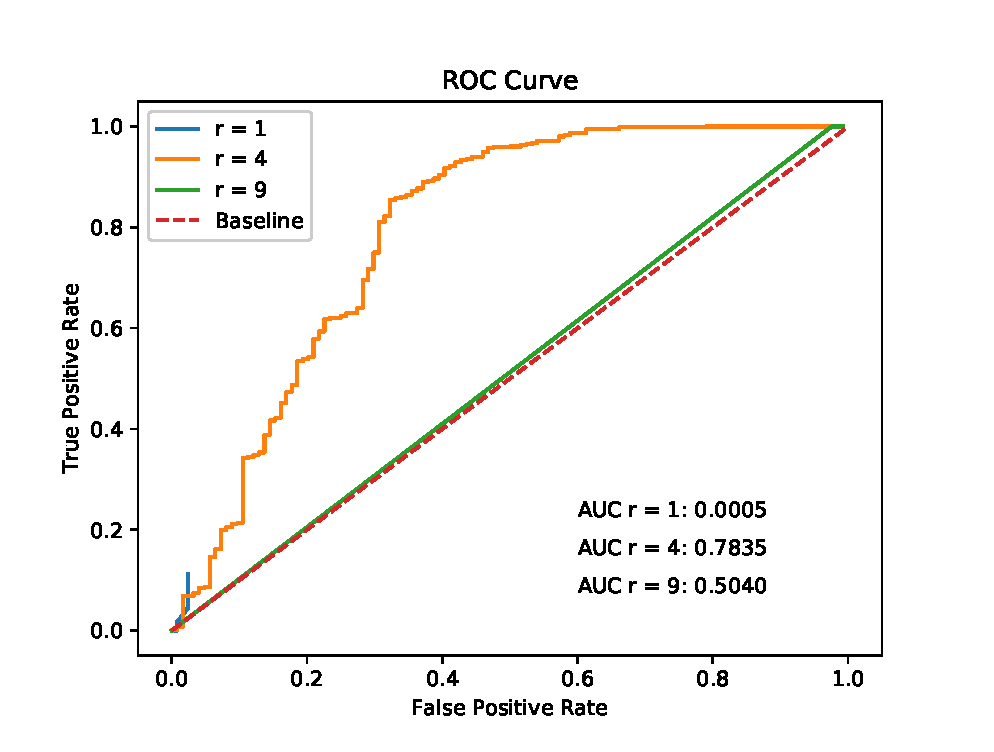
\includegraphics[width=0.7\textwidth]{images/roc_ex1.eps}
\caption{ROC curve for different values of $r$ in the negative selection algorithm}
\label{fig:ROC_ex1}
\end{figure}

\newpage

\item The ROC curve for differentiation of English and four other languages using the negative selection algorithm may be found in figure \ref{fig:ROC_ex1_3}. What we can see from this figure is that there is a clear ordering which language is discriminated best, since the ROC curves never cross paths, i.e. for every threshold it holds that languages have a constant ordering which is language is discriminated best. Judging from this figure \textit{Xhosa} is discriminated best, followed by respectively \textit{Hiligaynon}, \textit{Plautdietsch} and lastly \textit{Middle-English}.

I was actually suprised that all of the languages, exception being Middle-English, exist. However, upon closer inspection, this ordering makes sense. Middle-English is a precursor of English, so it shares similarities. \textit{Xhosa} is a Nguni Bantu language with `click consonants', so it makes sense that these languages are the most different and thus easiest to distinguish.

\begin{figure}[H]
\centering
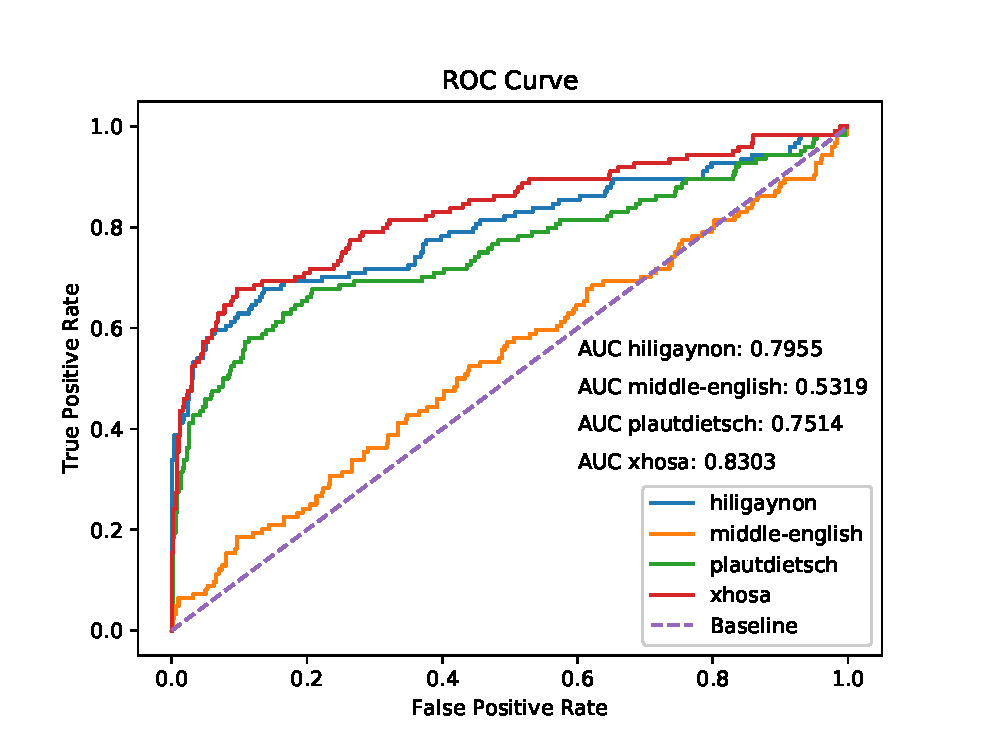
\includegraphics[width=0.7\textwidth]{images/roc_ex1_3.eps}
\caption{ROC curve for differentiation of English and four other languages using the negative selection algorithm.}
\label{fig:ROC_ex1_3}
\end{figure}

\end{enumerate}


\section{Intrusion Detection for Unix Processes}
\begin{itemize}
\item Detect anomalous sequences in the system calls datasets.
\item Do AUC analysis
\end{itemize}

\end{document}